% XeLaTeX + BibTeX. The mathematical blocks are shared with the Chinese edition.
\documentclass[11pt,a4paper]{article}
\usepackage{fontspec}
\setmainfont{Latin Modern Roman}
\setsansfont{Latin Modern Sans}
\setmonofont{Latin Modern Mono}
\tracinglostchars=3
\usepackage[a4paper,margin=23mm,headheight=15pt]{geometry}
\usepackage{amsmath,amssymb,mathtools,booktabs,tabularx,array,graphicx,xcolor,enumitem,fancyhdr}
\usepackage[numbers,sort&compress]{natbib}
\usepackage[unicode,hidelinks,breaklinks]{hyperref}
\usepackage{xurl}
\hypersetup{pdftitle={Candidate-Conditioned Teacher Scoring: A Systems Research Report},pdfauthor={Jiacheng Yu},pdfsubject={Historical teacher scoring source survey}}
\setlength{\parindent}{0pt}\setlength{\parskip}{0.45em}\setlength{\emergencystretch}{3em}
\setlist{nosep,leftmargin=1.5em}\renewcommand{\arraystretch}{1.16}
\newcolumntype{Y}{>{\raggedright\arraybackslash}X}
\newcommand{\code}[1]{{\small\nolinkurl{#1}}}
\pagestyle{fancy}\fancyhf{}\fancyhead[L]{\small Teacher scoring / research report}\fancyhead[R]{\small Historical snapshot}\fancyfoot[C]{\thepage}
% Shared equations are included by both language editions.
\newcommand{\ScoreEquations}{%
\begin{align}
z_{t,i} &= h_t^{\mathsf T} W_i+b_i,\\
\ell^{\mathrm{full}}_{t,i} &= z_{t,i}-\operatorname{LSE}_{j\in\mathcal V}z_{t,j},\\
\ell^{C}_{t,i} &= z_{t,i}-\operatorname{LSE}_{j\in C_t}z_{t,j}
=\ell^{\mathrm{full}}_{t,i}-\log Q_t(C_t).
\end{align}}
\newcommand{\KLEquations}{%
\begin{align}
p_i^C &= \frac{e^{z_i^S/\tau_S}}{\sum_{j\in C} e^{z_j^S/\tau_S}},\qquad
q_i^C = \frac{e^{z_i^T/\tau_T}}{\sum_{j\in C} e^{z_j^T/\tau_T}},\\
L_C &= \sum_{i\in C}p_i^C\log\frac{p_i^C}{q_i^C},\\
\frac{\partial L_C}{\partial z_j^S} &=
\frac{p_j^C}{\tau_S}\left(\log\frac{p_j^C}{q_j^C}-L_C\right),\quad j\in C.
\end{align}}
\newcommand{\Decomposition}{%
\begin{equation}
D_{\mathrm{KL}}(P\Vert Q) = D_{\mathrm{Ber}}(\alpha\Vert\beta)
+ \alpha D_{\mathrm{KL}}(P^C\Vert Q^C)
+ (1-\alpha)D_{\mathrm{KL}}(P^{\bar C}\Vert Q^{\bar C}).
\end{equation}}
\newcommand{\CounterExample}{%
\begin{equation}
P=(0.49,0.49,0.02),\quad Q=(0.005,0.005,0.99),\quad C=\{0,1\}.
\end{equation}}
\newcommand{\CostEquations}{%
\begin{align}
F_{\mathrm{dense}} &\approx 2RVd, & F_{\mathrm{selected}} &\approx 2RKd,\\
T &\gtrsim \max(F/P_{\mathrm{eff}}, B/\mathrm{BW}_{\mathrm{eff}})
+T_{\mathrm{launch}}+T_{\mathrm{validate}}+T_{\mathrm{pack}},\\
S_{\mathrm{request}} &= \frac{1}{(1-f)+f/s}.
\end{align}}

\begin{document}
\hypersetup{pageanchor=false}
\begin{titlepage}
\vspace*{11mm}{\small\sffamily\bfseries AI INFRASTRUCTURE / TECHNICAL REPORT}\par
\vspace{14mm}{\LARGE\bfseries Candidate-Conditioned\\[2mm]Teacher Scoring\par}
\vspace{6mm}{\large Systems context, probability contract, prior art and evaluation design\par}
\vspace{9mm}\hrule\vspace{7mm}
\begin{tabularx}{\linewidth}{@{}p{40mm}Y@{}}
Author & Jiacheng Yu\\
Edition & 29 October 2026; English\\
Measurements & At the historical snapshot, CPU numerical, gradient, GPU, HTTP and training experiments not run\\
\end{tabularx}
\par\vspace{10mm}\noindent\textbf{Scope.} This report studies a possible per-position candidate scoring contract for teacher inference. It records upstream behavior and mathematical limitations, not a measured speedup or a novel kernel claim. Experimental-status statements describe the c1ab1f4 snapshot; subsequent results are recorded separately.
\vfill{\small The reported code observations refer to frozen upstream revisions. Third-party results are not project measurements.}
\end{titlepage}
\hypersetup{pageanchor=true}
\section*{Abstract}
A post-training consumer may request teacher scores for different token sets at different causal positions. Whether a compact, candidate-conditioned path is useful depends on the consumer's exact loss, existing API semantics, causal alignment, and end-to-end costs. SGLang already offers per-item scoring and position selection; an open branch-specific pull request implements per-position IDs with full-vocabulary normalization. vLLM has merged a per-row interface, and IndexedLogits supplies an existing selected-logit primitive. Conditional reverse KL is not full-vocabulary KL, and the inspected Rethinking OPD implementation is not a drop-in consumer of conditional-only scores. These observations narrow rather than establish the potential contribution. No project numerical, GPU, service or training result was available at the historical snapshot.
\tableofcontents\clearpage
\section{Problem and research boundary}
On-policy distillation (OPD) can require teacher information on a student's trajectory. A sampled-token objective, teacher-top-$k$ loss, and student-top-$k$ conditional objective require different outputs. The request for student-top-$k$ renormalized reverse KL in verl is a concrete demand signal, not evidence that every training system needs this contract.\cite{verl6676,verlteacher,verlloss}

Let $R$ be the number of selected causal rows and $C_t$ the candidate IDs for row $t$. An API forced to use the union $U=\bigcup_t C_t$ may return $R|U|$ scores instead of $\sum_t |C_t|$. With uniform $K$ and little overlap, $|U|\leq\min(V,RK)$. This is an output-count model for that particular interface, not a measured byte reduction or a claim about every SGLang route.

Position selection, per-row candidate selection and normalization are separate concerns. Reducing returned scores alone does not establish reduced projection work; selected logits alone cannot reconstruct a full-vocabulary normalizer. A complete RL training benefit requires an actual, matched training measurement.
\section{Prior work and source snapshots}
At SGLang revision \code{4517a5ff1bbd1f944d6bde1819300ed14af7b698}, generic prefill logprob handling applies a request-level list across relevant rows. Its separate \code{/score} path accepts per-item label IDs and can renormalize over them; selected-position scoring also exists but still invokes dense readout. These are distinct mechanisms, so a blanket claim that SGLang lacks candidate or position selection would be false.\cite{sglangio,sglanglogprob,sglangscore,sglanglogits}

As observed on 29 October 2026, SGLang PR \#38119 is open against \code{sglang-miles}, not merged into the audited main revision, and preserves full-vocabulary normalization. vLLM PR \#56984 was merged on 3 October 2026 and already implements a per-row candidate interface. Both are prior art.\cite{sglang38119,vllm56984}

OmniLens and its IndexedLogits implementation already calculate selected per-row logits without a full gathered-weight intermediate. The primitive is not claimed as an invention here. The related Subset-KL implementation has different support and KL direction; a shared primitive does not make objectives equivalent.\cite{omnilens2026,indexedlogits,subsetkl}

Rethinking OPD studies student-top-$k$ behavior, Sparse Logit Sampling studies a different distillation setting, and Tail-Aware Top-$k$ OPD considers discarded probability mass. Their results are third-party observations and cannot be transferred as project benchmark results.\cite{rethinking2026,anshumann-etal-2025-sparse,tailaware2026}
\section{Mathematical contract}
For row $t$, let $h_t\in\mathbb{R}^d$, $W\in\mathbb{R}^{V\times d}$, $b\in\mathbb{R}^V$, and a nonempty set of unique IDs $C_t\subseteq\mathcal V$. An actual model may add scaling, softcaps or adaptation; those transformations must be preserved. The score definitions are:
\ScoreEquations
Here $Q_t(C_t)$ is teacher probability mass on the support. Exact full log-probabilities can be renormalized over $C_t$ because the common full normalizer cancels. Conversely, omitted logits can change full probabilities while selected logits remain unchanged.

For fixed support $C$, positive temperatures $\tau_S,\tau_T$ and a detached teacher, define student $p^C$ and teacher $q^C$:
\KLEquations
The derivative follows from the softmax Jacobian, $\partial p_i/\partial a_j=p_i(\mathbf 1_{i=j}-p_j)$. Unselected local logits have zero derivative under fixed support. Candidate selection itself is discrete; ties and support changes are outside this local derivative. Tied input/output weights and nonlinear readout introduce additional gradient paths.

Let $\alpha=P(C)$ and $\beta=Q(C)$, both strictly between zero and one. The exact decomposition is:
\Decomposition
Conditional KL omits support-mass mismatch and tail structure. A concrete counterexample is:
\CounterExample
Both conditional distributions are $(1/2,1/2)$, so conditional KL is zero, while full KL is positive. At $K=1$ the conditional loss and local gradient are identically zero; at $K=V$ the conditional and full objectives coincide. These are analytical statements, not numerical test results.
\section{Consumer and causal alignment}
At Rethinking OPD author-code revision \code{ac26e38d6f1572eb027597b48a9f4e01f6915ef8}, the inspected route uses full-normalized student and teacher log-probabilities for a log-ratio reward, normalizes support weights, and applies detached advantages through a PPO surrogate. A conditional-only teacher output changes that reward; it is not a loss-preserving substitute. The observation describes current inspected code, not the historical provenance of a paper figure.\cite{opdauthorcode,rethinking2026}

A practical integration must specify which policy generates $C_t$, when the IDs become available, tokenization and model revisions, and the next-token shift. Rollout-recorded support, a student prepass and reordered execution have different staleness and cost. At the historical snapshot, an actual consumer of the proposed direct conditional reverse KL had not been established.
\section{Architecture and potential change}
Figure~\ref{fig:arch} separates observed upstream operations, proposed components and existing prior art. A candidate branch would start before dense LM-head projection and provide an explicitly conditional output contract. A dense reference and any candidate implementation must agree on positions, ordered IDs, masks, normalization, transformations and error behavior. A full-normalized path remains distinct.
\begin{figure}[htbp]\centering
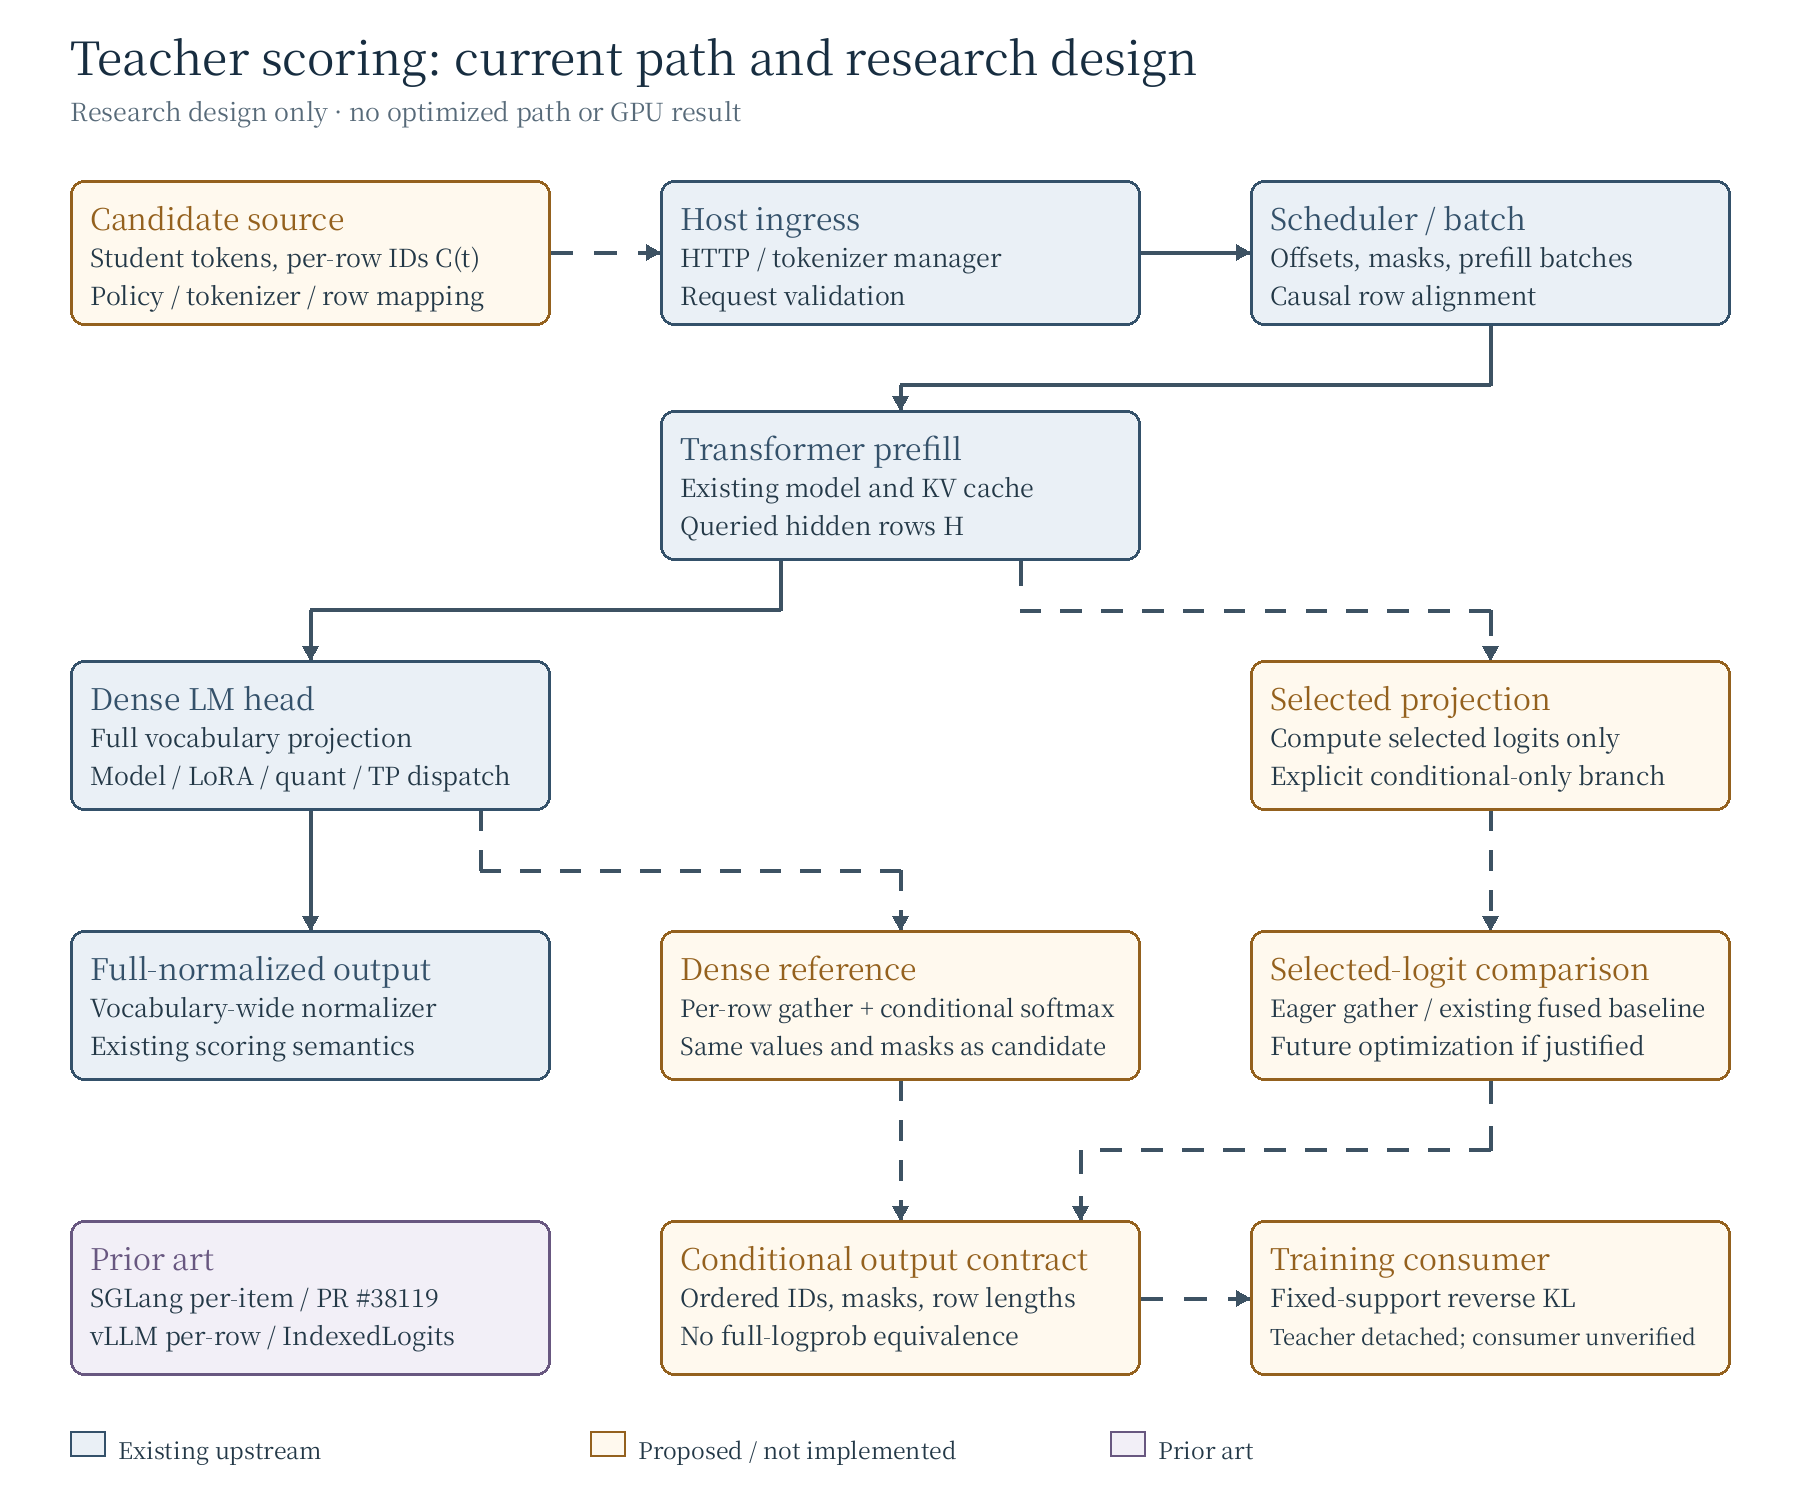
\includegraphics[width=0.92\linewidth,height=0.69\textheight,keepaspectratio]{docs/architecture/architecture.en.png}
\caption{Shared topology with English labels. Dashed proposed paths are not implemented.}\label{fig:arch}
\end{figure}
\section{Analytical cost model}
For uniform $K$, ignoring bias and other transformations, the approximate operation counts are $2RVd$ and $2RKd$. Effective time depends on achieved compute, memory traffic, launch, validation and packing. If an optimizable part takes fraction $f$ of a baseline request and is accelerated by factor $s$, Amdahl's relation gives the last expression:
\CostEquations
A FLOP ratio is not a latency prediction: dense matrix multiplication can reuse weights efficiently, while irregular gathers can waste bandwidth and incur launches. Existing model weights generally remain resident. Candidate overlap, batching and shape can change the preferred implementation.

\textbf{Analytical illustration only.} With $R=128$, $d=1024$, $V=131072$, $K=32$ and two-byte elements, head weights occupy 256 MiB, dense logits 32 MiB, an eager gathered-weight tensor 8 MiB and selected logits 8 KiB. These are tensor-size identities, not measured peak GPU memory. At hypothetical $f=0.1$, eliminating the affected part entirely bounds request speedup by $1/0.9$; actual $f$ is unknown.
\section{Evaluation design}
At the historical snapshot, all experiments below were proposed and \textbf{not run}. Compare a native full-normalized path only as context; for the same conditional contract compare dense projection plus gather, chunked dense, eager indexed gather and the existing IndexedLogits implementation when compatible. A future candidate must beat strong correct baselines on relevant workloads, rather than only the slowest baseline.

Start with CPU FP64 references for logits, normalization, loss and student gradients. Test $K=1$, $K=V$, permutations, invalid or duplicate IDs, ragged rows, masks, omitted-logit changes and causal off-by-one cases. Declare tolerances and quantized input values before comparing implementations. Teacher values must be detached. Unsupported LoRA, quantization or tensor-parallel modes need explicit rejection or a semantics-preserving, measured fallback.

For performance, freeze hardware, driver, framework, model and tokenizer revisions, traces, dtype, masks, batching and timing boundaries. Include low/high candidate overlap, representative row counts and prompt lengths, feasible concurrency, and OOM/fallback cases. Establish stable A/A controls before randomized paired A/B blocks; preserve failures and negative outcomes. Measure kernel and complete HTTP request latency separately, including p50/p95, throughput, memory, payload bytes and error rates. Profile outside headline timing. A teacher-only replay is not a full training run.
\section{Limitations and decision criteria}
At the historical snapshot, the exact real consumer and any remaining gap relative to the cited APIs and kernels were unresolved. No project CPU numerical, gradient, GPU, HTTP or real training experiment had been performed. There was no evidence of project speedup, memory saving, training quality benefit or a novel selected-logit primitive. A gap is credible only with a concrete consumer, fixed semantics and a reproducible comparison against relevant existing paths. Record an inconclusive or negative result when those conditions fail.

The source survey is bounded to the cited snapshots, not an exhaustive novelty search. Upstream source and papers remain attributed to their authors; no third-party implementation is vendored here. The inspected IndexedLogits repository did not declare a license in the reviewed files, so later reuse requires separate permission analysis.
\section{Document reproduction}
From the repository root, install XeLaTeX, BibTeX, Poppler, Python and Pillow, and use the bundled font subset as documented in the README. Run \code{bash scripts/build_assets.sh} and \code{python3 scripts/verify_assets.py}. This rebuilds document assets only; it does not execute SGLang or benchmark the research hypothesis.
\bibliographystyle{plainnat}
\bibliography{docs/reports/references}
\end{document}
